% -*- Mode: LaTeX; Mode: visual-line; -*-
\documentclass[E]{compsoft}


\taikai{2019}
\pagestyle {empty}

\usepackage [dvipdfmx] {graphicx}

% ユーザが定義したマクロなどはここに置く.ただし学会誌のスタイルの
% 再定義は原則として避けること.

\begin{document}

\title{ASTToken2Vec: an Embedding Method for Neural Code Completion}

\author{Dongfang Li  \quad   Hidehiko Masuhara
%
% ここにタイトル英訳 (英文の場合は和訳) を書く.
%
\ejtitle{ASTToken2Vec: 神経回路網によるコード補完のための埋め込み手法}
%
% ここに著者英文表記 (英文の場合は和文表記) および
% 所属 (和文および英文) を書く.
% 複数著者の所属はまとめてよい.
%
\shozoku{李 東方, 増原 英彦}{東京工業大学数理計算科学系}%
{Department of Mathematical and Computing Science, Tokyo Institute of Technology}}




\Eabstract{
Code completion systems help the programmers to write code more efficiently and to reduce typographical errors by automatically suggesting code fragments that the programmers likely to write next. This work attempts to improve an LSTM neural network-based code completion system by proposing a new embedding method called ASTToken2Vec for program tokens. ASTToken2Vec is inspired by Word2Vec, and gives a vector representation to a program token so that tokens often appear in similar contexts are mapped to positions close to each other.  We integrated ASTToken2Vec with the LSTM-based code completion model and evaluated its prediction performance by using a dataset consisting of 150,000 open-source JavaScript program files.}
\maketitle \thispagestyle {empty}







\section{Introduction}
% what is code completion system, why it is useful.
Code completion is a feature of programming editors that suggests code fragments that are likely to be typed in by the programmer following to the program text just before the cursor position.  It helps the programmer to write code more quickly, to remember rarely used API names, and to reduce typographical errors.

% Define prediction context
In general, code completion systems make suggestions (we hereafter call \emph{predictions}) based on the program text around the cursor position (we hereafter call a \emph{context}).  Predictions are usually a list of identifiers (e.g., function, method and variable names), but some systems predict a sequence of tokens or a few lines of statements.

% problems in traditional code completion
Context information determine the prediction performance.  For example, a standard completion feature in Eclipse JDT merely the type of the receiver expression as the context when it predict a method name of a method invocation expression.  Eclipse code recommender \cite{heinemann2011suite} additionally uses a sequence of method calls preceding to the cursor line as the context.  It can improve prediction 
since many libraries require client programs to call several functions/methods in specific orders.

Traditional code completion systems make limited use of context information.  For example, Eclipse code recommender, while it uses preceding method calls, ignores names of local variables and control flow around the cursor position.  It also ignores of calls of methods defined in the current project as it relies on the knowledge of the usages of well known libraries.

% First, they 
%  make limited use of contexts.  As mentioned above, they tend to use 
% Most of them are based on statistical methods and suggest code only by simple term frequency which often relatively have a higher error rate. 
% Another problem is that they rely on static types (like Eclipse for Java) to filter out candidates. 
% However, the dependency on typing information limits their applicability to widely used in dynamically typed languages like Python.etc.

% deep learning models, the reason we can apply dl model to code completion
Deep learning-based code completion, which is actively studied in the last few years, takes a different approach to exploit context information as well as knowledge of the programming language and APIs.  
It uses a neural network model, more specifically, a recurrent deep neural network (RNN) that takes a sequence of program tokens and predicts the next token.  RNNs are known to be successful in the domain of natural language texts. 

When applying an RNN (LSTM?) to programming languages, SOMEONE proposed to encode structural information of a program in addition to the lexical tokens that form the program.  *****(write more)

\begin{figure}[!ht]
\centering
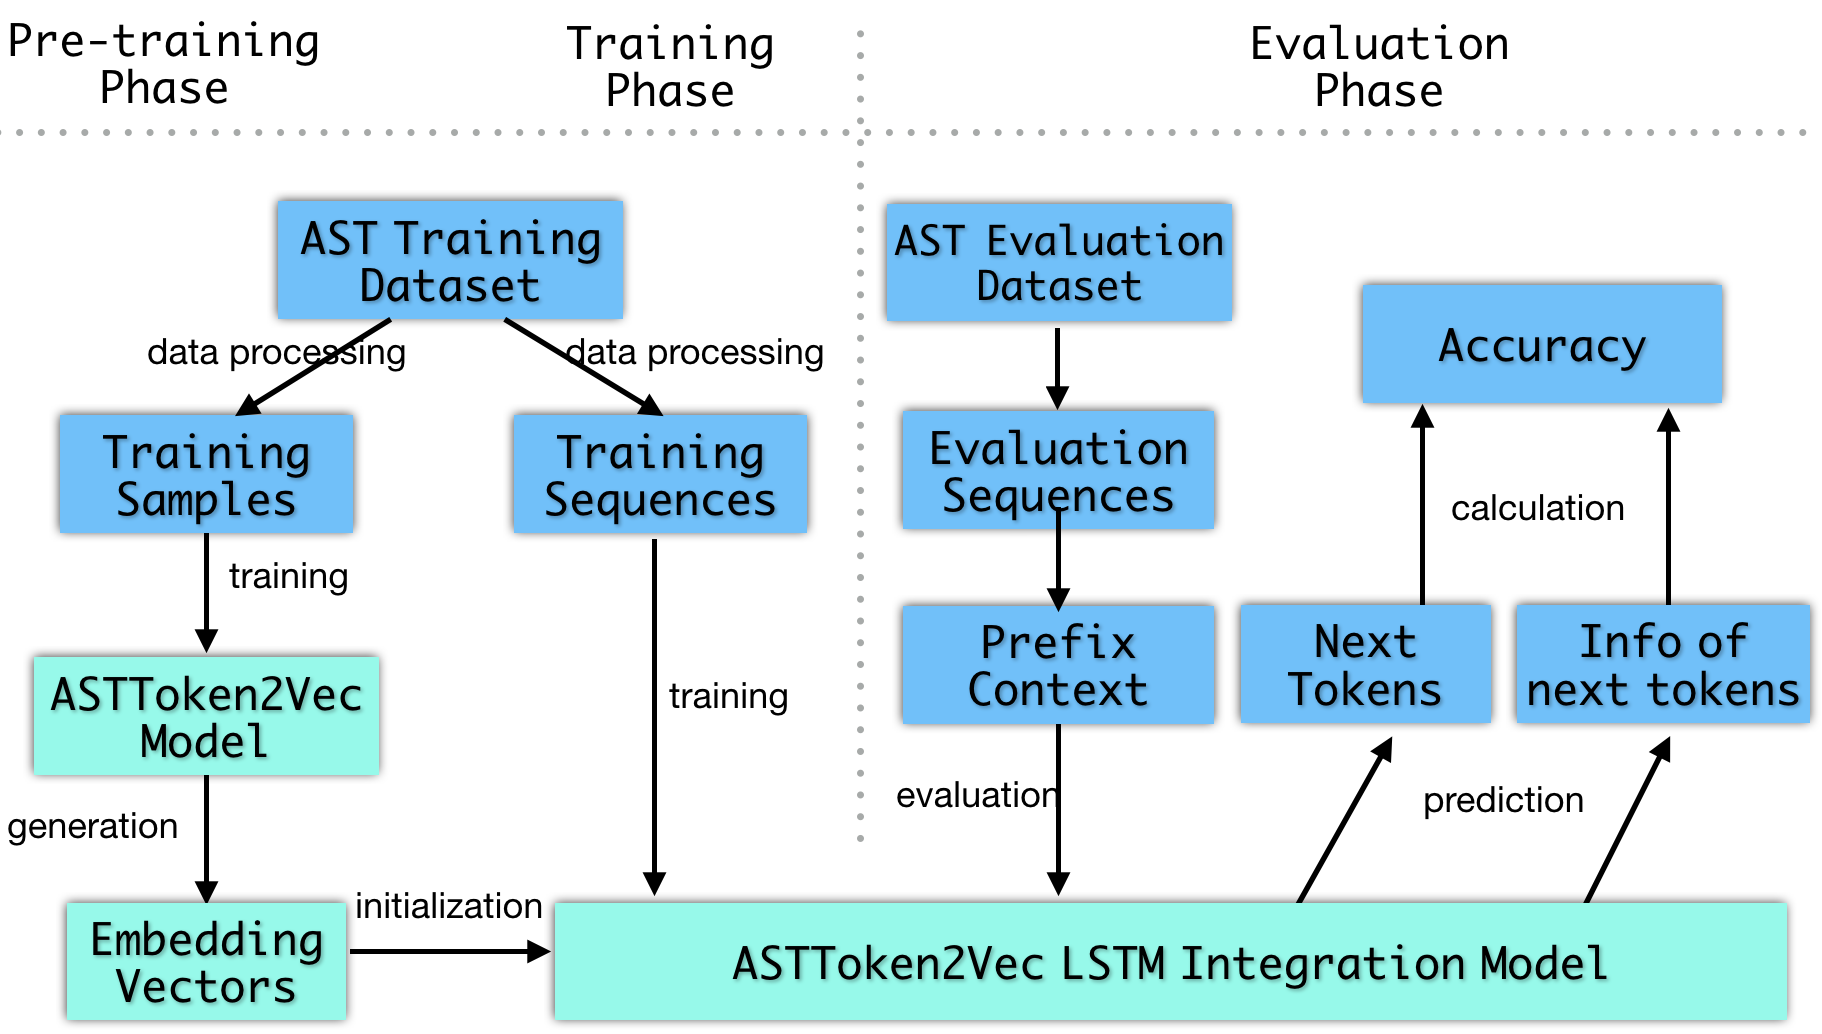
\includegraphics[width=7.5cm, height=5.5cm]{pictures/model_overview.png}
\caption{Overview of ASTToken2Vec LSTM integration model}
\label{fig:overivew_model}
\end{figure}
% introduce our work: node2vec 
% The embedding method is a way to represent discrete variables as continuous vectors. 
This paper proposes an embedding method called ASTToken2Vec for abstract syntax tree (ASTs) nodes of a program in order to improve the prediction performance of the deep learning-based code completion. 
It is a four-layer neural network that takes one AST token along with a few contextual tokens as input, and outputs one vector that represents the AST token.  The intuition behind the embedding is to give similar vector representation for the tokens that are semantically similar, which is similar to the idea behind the Word2Vec embedding \cite{word2vec}.
As a code completion system, whose overview is shown in Figure~\ref{fig:overivew_model}, we use the embedding method as a pre-trained frontend to an LSTM-based neural network that predicts next AST token from a sequence of AST tokens.
% The vector representation will be used to learn and predict in a code completion system called the AT2V-LSTM model.  
% to learn and encode context information of AST tokens to generate semantic-based embedding representation vectors that contain more knowledge hidden behind ASTs. 
% We use this ASTToken2Vec model as a pre-trained model and integrate it with an LSTM based model as a code completion system to predict next tokens. 
% We name our integration model as AT2V-LSTM model and the overview of our model illustrates in Figure \ref{fig:overivew_model}.

As an experiment, we implement both ASTToken2Vec embedding and AT2V-LSTM model with a JavaScript AST dataset\Cite{dataset} collected from open-source programs containing a total of 150,000 JavaScript files. 
We visualize representation vectors of several terminal tokens and evaluate the performance of predicting next tokens by AT2V-LSTM integration model.
From the results analysis, we conclude that the ASTToken2Vec method is able to generate semantic-based representation vectors of AST nodes and the AT2V-LSTM integrated model predicts tokens more accurately.




\section{Background}
% This is related work.  (issue #3)
Hindle et al.\  \cite{hindle2012naturalness} used the \textit{n-gram} technique for code completion.  Their work showed that programming code is more repetitive than natural language texts.
% this is also related work: TODO: read the paper
Nguyen et al.\  \cite{DBLP:journals/corr/MaddisonT14} propose generative models of natural source code with hierarchical structure and a distributed representation of source code element. 
They also leverage compiler logic and abstractions to improve their generative models.
% this is also related work.
Tung et al.\  \cite{Nguyen:2013:SSL:2491411.2491458} extends the state-of-the-art \textit{n-gram} approach which is called SLAMC by incorporating semantic information into code tokens. 

% related work, as it is statistical
Allamanis et al.\ proposed a statistical nonparametric Bayesian probabilistic tree-based system for extracting programming idioms from a source code text
\cite{allamanis2014mining}.
% related work, TODO cannot understand...
Liang et al.\  \cite{liang2010learning} focus on learning programs for multiple related tasks with a few training samples and propose a nonparametric hierarchical Bayesian model which is able to share the statistical information across multiple tasks for code completion.

% related work, TODO what is "by allowing conditioning of a production rule. "???
Bielik et al.\  \cite{bielik2016phog} proposed a generative model for code called the probabilistic higher-order grammar. This model can capture context information between tokens by allowing conditioning of a production rule. 
% this is ...? a subsequent work of raychev2014code, background???
Raychev et al.\  \cite{raychev2016probabilistic} create a domain-specific language (DSL) over abstract syntax trees (ASTs) called TGEN which can encode an AST to a specific language context.
They also propose a special decision tree called DEEP3 which can make code predictions leveraging the AST context encoded by the TGEN model.

% Raychev is RNN but we do not directly based on this!???
Raychev et al.\  \cite{raychev2014code} and White et al.\  \cite{white2015toward} explore how to apply RNN models on sequences of tokens to facilitate the task of code completion.
% This is the work we based on.  Hmm, it is a rejected paper.
Liu et al.\  \cite{liu2016neural} propose several LSTM-based models for code completion with an AST dataset and they leverage the ASTs by converting ASTs to sequences of training samples. 
Their work gives us inspiration about how to convert an AST to a sequence and how to train an LSTM model with AST dataset. 

% TODO: tree encoding
% TODO: Word2Vec


\section{Abstract Syntax Tree}
% 介绍AST的详细内容,结构等
An abstract syntax tree (AST) is a structure that represents structural information of programs. It is widely used in code completion.
%ASTToken2Vec model training and AT2V-LSTM integration model training.

% this is background information
An AST consists of two kinds of nodes, namely \emph{non-terminal nodes} and \emph{terminal nodes}.
A non-terminal node is a node that has one or more children nodes. 
For example, in JavaScript, non-terminal nodes correspond to syntax categories such as function declarations, variable declarations, \texttt{for} statements, \texttt{if} statements, and \texttt{while} statements.
% These non-terminal tokens declare what kind of functions or variables specified in the program. 
% Other kinds of non-terminal tokens represent more knowledge about the structure and logical judgment of a program like ``ForStatement'', ``IfStatement'', ``WhileStatement'', etc. 

A terminal node is a node that appear only at leaf positions in an AST.
We call the lexical token of a terminal code as a \emph{value}.
In JavaScript, terminal nodes correspond to to syntax categories such as identifiers (variable, field and function names), literal numbers, and literal strings.  

% Due to ASTs contain more semantic knowledge about source code, we use ASTs as the basic data to generate two sets of training samples for our models' training.



\section{ASTToken2Vec Embedding}
\label{section:node2vec}
ASTToken2Vec is an embedding neural network model for AST nodes.  By using ASTToken2Vec, we convert between program tokens and a point in a vector space so that the latter representation can be used as input/output of the neural network model for code completion.  

Intuitively, we design ASTToken2Vec to incorporate similarities of tokens into embedded representations, where two similar programs tokens will have two points in the vector space that are close to each other.  By similarity, we here mean similarity in natural language semantics (such as ``\texttt{size}'' and ``\texttt{length}'') as well as similarity in the API usage (such as \texttt{Stack.peek()} and \texttt{Stack.pop()}).

ASTToken2Vec is inspired by Word2Vec \cite{word2vec}, which gives vector representations to natural language words. Differently from Word2Vec, ASTToken2Vec 
uses two identical networks for embedding non-terminal and terminal tokens.  It also separately provides non-terminal and terminal tokens as context information for training.

% ASTToken2Vec trains a four-layers neural network to generate the semantic-based representation vectors of AST nodes which enable the LSTM-based code completion model to leverage more structural knowledge to predict next tokens.
% In order to do that, we give a basic hypothesis of ASTToken2Vec which is same as Word2Vec's: we assume that if two nodes in an AST have a similar context, the meaning of these two nodes also has a high-level similarity. 
% We specified the surrounding non-terminal nodes of a target node as the non-terminal context and surrounding terminal nodes as the terminal context. The details of contexts is explained in subsection\ref{sub:embedding_nt} and subsection\ref{sub:embedding_tt}.


\subsection{Model Architecture}
\begin{figure}[!ht]
\centering
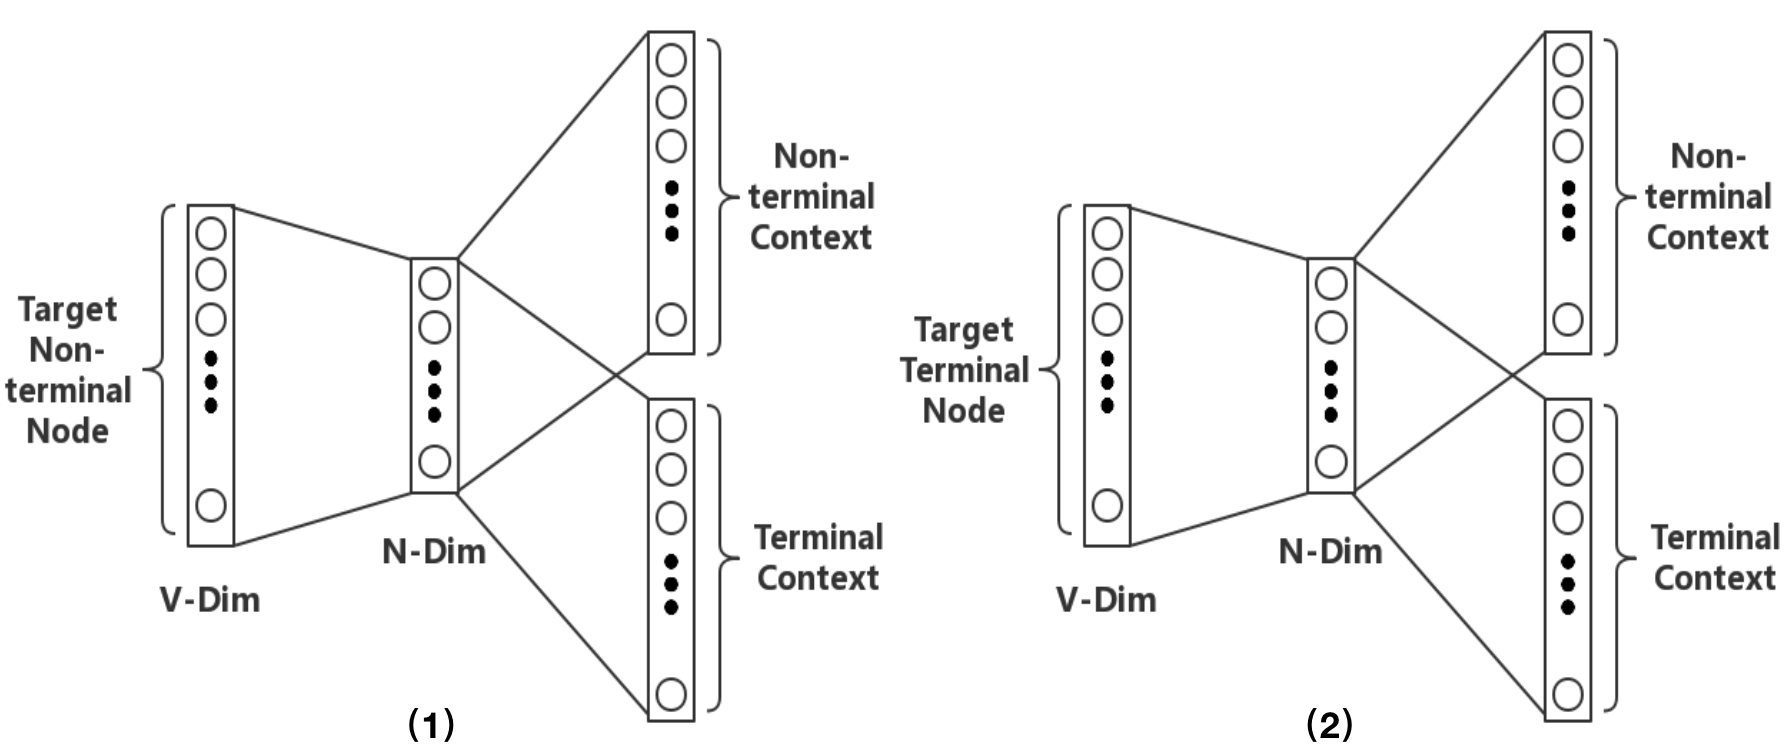
\includegraphics[width=7.5cm, height=4cm]{pictures/node2vec_structure.png}
\caption{Architecture of NT2V (1) and TT2V (2)}
\label{fig:node2vec-structure}
\end{figure}
ASTToken2Vec is a pair of four layers neural networks, each contains one input layer, one hidden layer, and two output layers as shown in Figure~\ref{fig:node2vec-structure}.  Two identical, yet independent networks are for embedding non-terminal and terminal nodes, respectively.  We hereafter call the networks NT2V and TT2V, respectively.

The input layer uses the one-hot encoding representation, where $i$'th token in a vocabulary of $V$ different tokens is represented as an $V$-dimensional vector all but $i$'th element is zero.  
The two output layers represent the context of non-terminal and terminal nodes, each of which has the same vector size to the non-terminal/terminal input vectors.
We use the values in the hidden layer as the embedding vector of the input values.  The size of the hidden layer, a hyperparameter $D$, is determined by heuristics.
In the training phase, we calculate a joint loss function to update the model.

% Figure \ref{fig:node2vec-structure}(1) illustrates the architecture of the NT2V model and Figure \ref{fig:node2vec-structure}(2) is the architectrue of TT2V model.



\subsection{Embedding for Non-terminals (NT2V)}
\label{sub:embedding_nt}
The NT2V embedding uses both the terminal and non-terminal contexts for training.
A training tuple for NT2V contains three elements: (\textit{target non-terminal, non-terminal context, terminal context}) where the \textit{target non-terminal} is the non-terminal token which the NT2V model generates embedding vector for. 
The second and third elements are lists representing the contexts of the input \textit{target non-terminal}.
We define these two contexts as follows.

\subsubsection{Non-terminal context}
The non-terminal context for a non-terminal token means the surrounding non-terminal nodes of it in an AST. ****************
Concretely, we define the $n$ parent non-terminal nodes of a target non-terminal and its all non-terminal children nodes as its non-terminal context.
Here, $n$ is a hyper-parameter which declares the scope of the parent non-terminal context employed by the NT2V model. 
If $n$ is relatively small, it means NT2V model does not consider the surrounding non-terminal tokens which are far from the target node as the non-terminal context.

\subsubsection{Terminal context} 
We define the terminal context of a target non-terminal as all its children terminal nodes. 
If a non-terminal node does not have any terminal children nodes (all its children nodes are non-terminal tokens or it does not have any children), we use a special terminal token: \textit{TT-EMPTY} to declare an empty terminal context for it.

We use an example of partial AST to illustrate the contexts of a non-terminal in the Figure \ref{fig:node2vec-context}(1). The nodes whose name starts with ``NT'' are non-terminal nodes and nodes whose name starts with ``TT'' represent terminal nodes. 
In this AST, We assume a target non-terminal node ``NT-4'' which is surrounded by an oval. 
Non-terminal nodes surrounded by a rectangle are the non-terminal context of the target node including ``NT-2'' and ``NT-1''. 
Terminal nodes: ``TT-1'', ``TT-2'' and ``TT-3'' which have an underline mean the terminal context of the target node ``NT-4''. 
Hyper-parameter $n$ here is specified as two.


\begin{figure}[!ht]
\centering
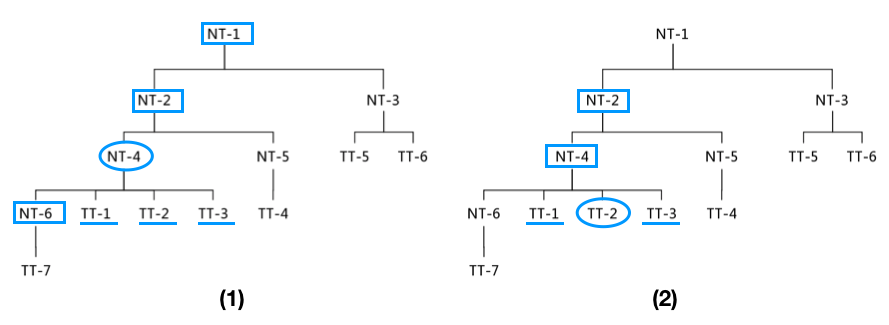
\includegraphics[width=7cm, height=3.5cm]{pictures/node2vec_context.png}
\caption{Non-terminal and terminal context for non-terminal nodes (1) and terminal nodes (2)}
\label{fig:node2vec-context}
\end{figure}





\subsection{Embedding for Terminals}
\label{sub:embedding_tt}
The ASTToken2Vec model for terminal tokens' embedding vectors generation is abbreviated as TT2V.
Similar with NT2V model, the structure of training tuples for TT2V is (\textit{target terminal, non-terminal context, terminal context}) 
NT2V model leverage both non-terminal context and terminal context to generate the embedding vectors for the \textit{target terminal}.
The non-terminal context and terminal context of a target terminal are described as below.

\subsubsection{Non-terminal context} 
Because there is no child node of a terminal node, we only consider the non-terminal context of a terminal as only its $n$ parent non-terminal nodes. 
Same with NT2V, hyperparameter $n$ is used to define the scope of non-terminal context.

\subsubsection{Terminal context} 
We define the terminal context of a target terminal node as $m$ neighbor terminal nodes in an AST. 
Neighbor terminal nodes of a target terminal mean its sibling terminals which have the same parent non-terminal with the target terminal.
Here $m$ is a hyperparameter to specify the size of the terminal context. 
A relatively small $m$ means TT2V model does not consider too many surrounding terminal nodes as the terminal context. 
If a terminal node does not have any neighbor terminal nodes which means its parent node only has one single terminal child, in this case, we use a special terminal node: \textit{TT-EMPTY} to represent an empty terminal context. 

The partial AST in the Figure \ref{fig:node2vec-context}(2) shows a concrete example of what is contexts for terminals.
We specify a target terminal node ``TT-2'' which is surrounded by an oval. 
Non-terminal nodes: ``NT-2'' and ``NT-4'' which are emphasized by a rectangle, represent the non-terminal context and terminal nodes ``TT-1'' and ``TT-3'' are the terminal context of the target node. 
In this example, hyperparameter $n$ is specified as two and $m$ is equal to one.

\subsection{Joint Loss Function}
Due to there are two output layers in our ASTToken2Vec model, we design a joint loss function combining the non-terminal context output and terminal context output. 

There are three parts of the loss function calculation. 
$Loss_{nt}$ is used to represent the loss of non-terminal context output. 
The loss of terminal context output is represented by $Loss_{tt}$. 
Both of them are multi-labels loss calculations because there are more than one surrounding tokens as the context. 
And $Loss_{total}$ is the final joint loss function for our model's training.

\begin{equation}
Loss_{nt} = -\sum_{i=1}^{N}(y_{nt-context}^{i} \times log(\hat{y}_{nt-context}^{i}))\label{equ:lossnt}
\end{equation}

Equation\ref{equ:lossnt} is the $Loss_{nt}$ calculation formula which is a $log$ loss function. 
Concretely, for an input token $x$, ASTToken2Vec model calculates the non-terminal context output as $\hat{y}_{nt-context}$ and $y_{nt-context}^{i}$ represents its ground-truth non-terminal context.
$N$ is the size of the non-terminal vocabulary. 


\begin{equation}
Loss_{tt} = -\sum_{j=1}^{M} (y_{tt-context}^{j} \times log(\hat{y}_{tt-context}^{j}))\label{equ:losstt}
\end{equation}

Equation\ref{equ:losstt} illustrates the formula of $Loss_{tt}$ calculation which also a $log$ loss function. 
$\hat{y}_{tt-context}$ is the terminal output of our model. and $y_{tt-context}$ is the ground truth label of the terminal context.
$M$ is the size of terminal vocabulary.

\begin{equation}
Loss_{total} = \alpha * Loss_{nt} + (1-\alpha) \times Loss_{tt}\label{equ:totalloss}
\end{equation}

Equation\ref{equ:totalloss} is the joint loss function combining $Loss_{nt}$ and $Loss_{tt}$. 
We utilize a hyperparameter $\alpha$ whose range is from zero to one to adjust the importance between the loss of non-terminal context output $Loss_{nt}$ and terminal context output $Loss_{tt}$.




\section{AT2V-LSTM Integration}
\label{section:n2v-lstm-integration}
We integrate a basic LSTM model with our ASTToken2Vec embedding method. This integration model is called AT2V-LSTM which is able to leverage the semantic-based information extracted by ASTToken2Vec embedding and predict the next tokens as code completion.


\subsection{Sequences of Training Samples}
In order to train the linear-structured LSTM model, we convert ASTs to sequences of training samples.
Basically, we first convert an AST to a left-child-right-sibling (LC-RS) binary tree. 
Then, we transform this LC-RS binary into a complete binary tree by padding a special non-terminal node \textit{NT-EMPTY}.
Next, we apply a deep-first in-order traversal on this complete binary tree to generate a visiting sequence of training samples. 
There are four elements in a sample: (\textit{non-terminal, terminal, node-or-leaf, right-or-left}).
Concretely, when a non-terminal node is visited, it is considered as a target \textit{non-terminal} and the first element in the sample.
The second element: \textit{terminal} is the children terminals of the target \textit{non-terminal}.
If the target \textit{non-terminal} does not have any terminal child, we use a specified terminal token \textit{TT-EMPTY} to represent its empty child.
The last two elements: \textit{node-or-leaf} is used to declare whether the \textit{non-terminal} is a leaf or not in the complete binary tree and \textit{right-or-left} represents the position relationship between the target \textit{non-terminal} and its parent node. 
These two elements are used to reconstruct the predicting AST from the sequence of training samples.



\subsection{Model Architecture}
The architecture of our integration model is illustrated in the Figure \ref{fig:nti2p_model_architecture}. 
It contains one input layer, one LSTM layer, and an output layer. 


\begin{figure}[!ht]
\centering
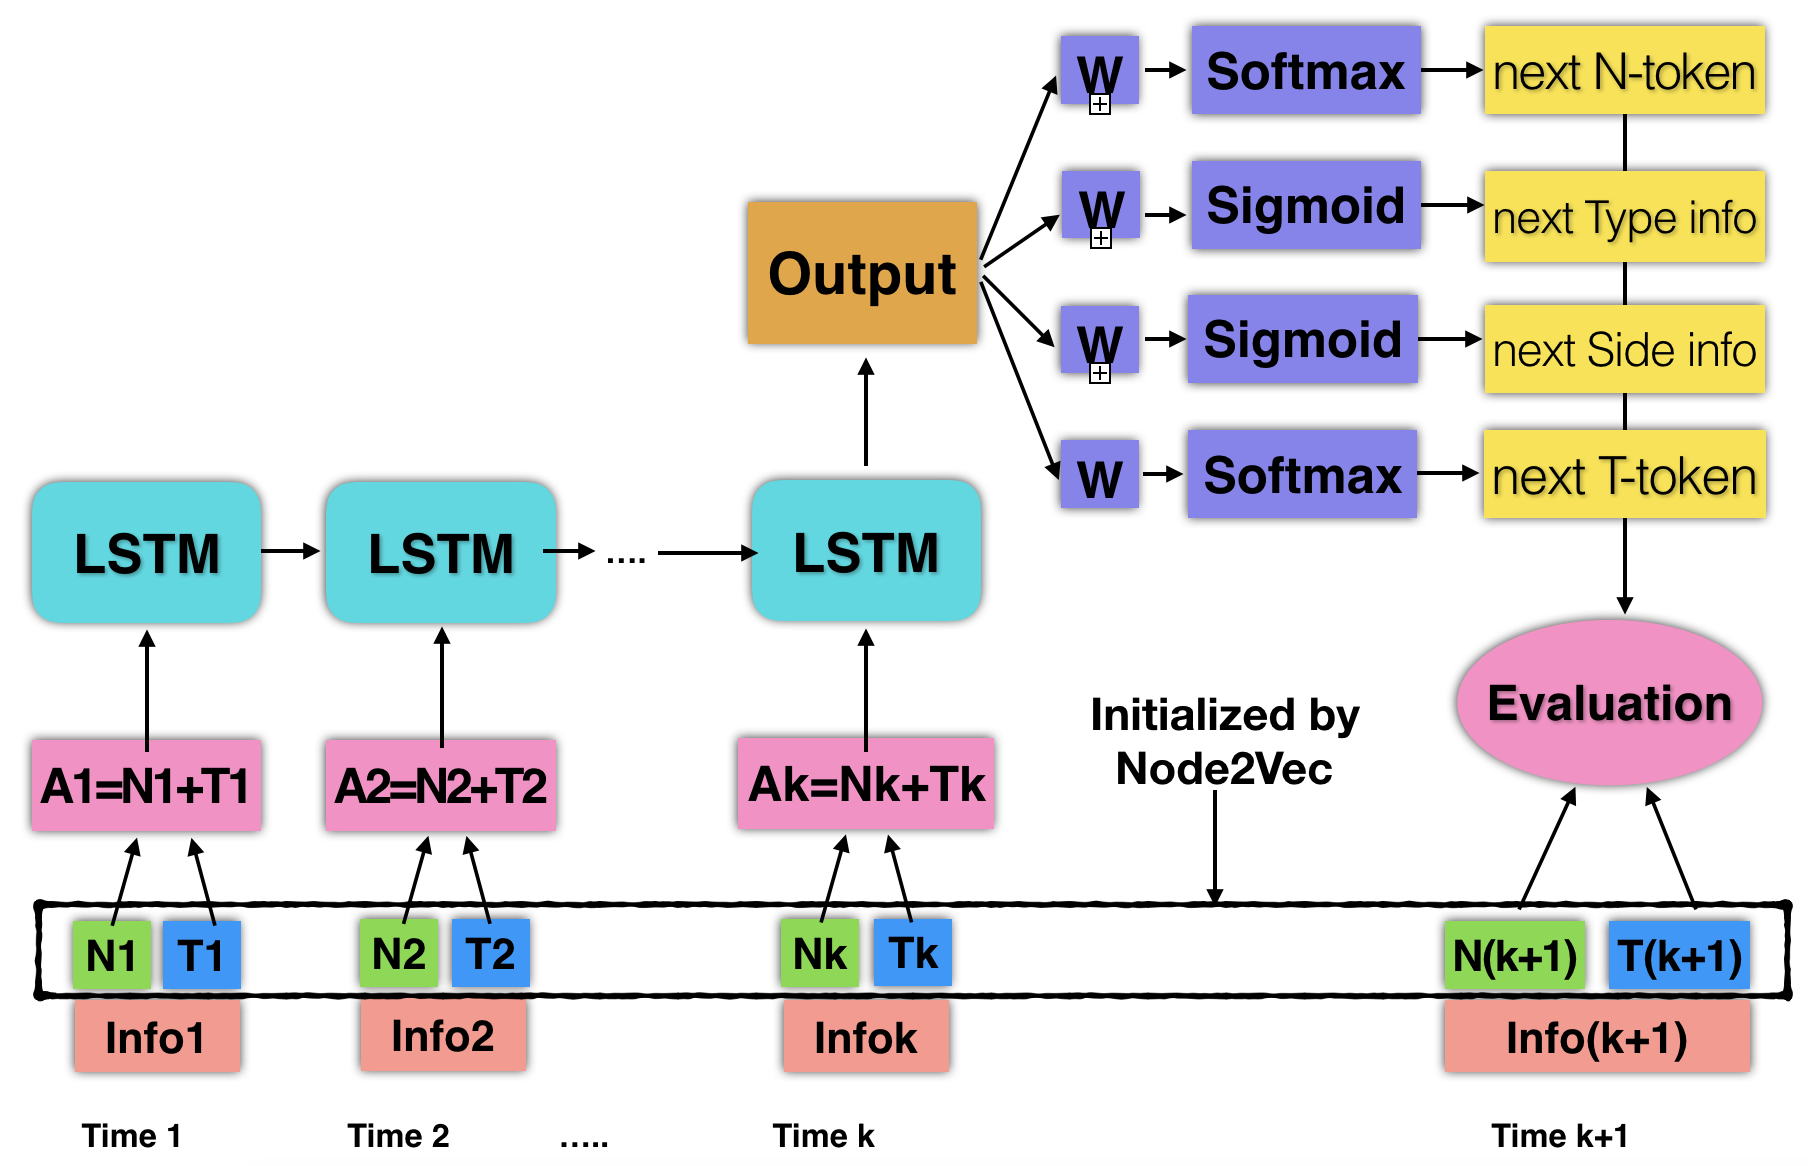
\includegraphics[height=4cm, width=7.5cm]{pictures/lstm_structure.png}
\caption{The architectrue of AT2V-LSTM model}
\label{fig:nti2p_model_architecture}
\end{figure}


\subsubsection{Input layer}
The input layer is a combination layer of the representation vectors of feeding elements and these vectors are initialized by ASTToken2Vec embedding.
The input is a sequence of training samples and one sample has four elements: $(N_{i}, T_{i}, NL_{i}, RL_{i})$ where $N_{i}$ is a non-terminal, $T_{i}$ is a terminal, $NL_{i}$ is the type information of $N_{i}$ and $RL_{i}$ is the side information of $N_{i}$. All these four elements are encoded by one-hot encoding and multiply embedding matrices as below:

\begin{equation}
Input_{i} = Concat(A\cdot N_{i} + B\cdot T_{i}, \quad C\cdot NL_{i} + D\cdot RL_{i})\label{equ:input}
\end{equation}

where $A, B$ are the embedding matrices for non-terminals, terminals and initialized by embedding vectors generated by ASTToken2Vec. $A$ is a $K \times V_{N} $ matrix and the shape of matrix $B$ is $K \times V_{T}$. $K$ is the length of embedding vectors. 
$V_{N}$ and $V_{T}$ are the size of non-terminal vocabulary and terminal vocabulary respectively. 
$C, D$ are embedding matrices for type information, and side information.
% initialized randomly. 
%The shape of $C$ and $D$ is $J \times 2$ where $J$ is the length of embedding vector for $NL_{i}$ and $RL_{i}$.


\subsubsection{LSTM layer}
The LSTM layer receives the embedding vectors from the input layer as $x_{i}$ and takes the output $h_{t-1}$ and hidden state $c_{t-1}$ from the previous state of LSTM layer. 
Then, the LSTM layer computes three operating gates: forget gate, update gate and output gate to calculate a new hidden state as $h_{t}$ and the new output as $c_{t}$.



\subsubsection{Output layer}
The output layer has four trainable matrices as the linear mapping between the output of the LSTM layer and the prediction. 
There are four instances our model predicting: 
next non-terminal $N_{i+1}$, next terminal $T_{i+1}$, type and side information of the next non-terminal, $NL_{i+1}$ and $RL_{i+1}$. 
The formula of output layer is as below:

\begin{equation}
P_{i} = softmax(W \times h_{i} + b)
\end{equation}


where $P$ is the prediction of next training sample including $p_{n}, p_{t}, p_{nl}$ and $p_{rl}$ representing the prediction of next non-terminal, next terminal, the side and type information of $p_{n}$. 
$W$s are four trainable matrices for linear mapping and $h_{i}$ is the output of the LSTM layer.
The softmax function returns the possibility of the next tokens predicting.
 




\section{Experiments}
\label{section:experiment}
\subsection{Dataset Details}
The data we use for both the ASTToken2Vec embedding model training and AT2V-LSTM integration model training is from the same dataset which is a JavaScript AST dataset provided by Raychev et al.\  \cite{dataset}. 
There are 100,000 ASTs as training dataset and 50,000 ASTs as evaluation dataset. 

% 介绍nonterminal的数据集,并解释增加了两个新bit,扩展了nonterminal的种类
\subsubsection{Non-terminal Vocabulary} 
There are 44 different kinds of non-terminal tokens specified by the JavaScript programming language grammar. 
Base on these 44 non-terminals, we add two more bits of information: whether the non-terminal token has a child token; whether this non-terminal has a right sibling or not. 
These two bits care more about the surrounding context of non-terminals and make the task of non-terminal predict become more challenge. 
This adjunction is also used in the previous work\cite{liu2016neural}\cite{dataset}. 
There are 98 kinds of bits-information combination non-terminal tokens in total as the elements in the non-terminal vocabulary including the special non-terminal token:\textit{NT-EMPTY} we use as a padding token to build a complete binary tree from an AST.

\subsubsection{Terminal Vocabulary} 
Theoretically, there are infinite kinds of terminal tokens may be included in programs.
So, we use the idea of \textit{Word of Bag} to specify the terminal vocabulary. 
Concretely, we sort all terminal tokens appearing in the training dataset by their frequencies of occurrence. 
Then we choose the 50,000 most frequent terminal tokens as the vocabulary of the terminal. 
For infrequent terminal tokens (out of our terminal vocabulary bag), we use a special terminal token \textit{UNK} to represent these terminals. 
In total, we have 50,002 tokens in the vocabulary of the terminal including particular terminal \textit{UNK} and \textit{TT-EMPTY} which is used to represent a child terminal for a non-terminal who does not have a terminal child. 



\subsection{Experiment of ASTToken2Vec}
\subsubsection{Training details}
We implement ASTToken2Vec models to generate embedding vectors for both non-terminals and terminals. We define the size of the hidden layer $D$ is equal to 1,000 so that the length of embedding vectors is 1,000. 
We specify the adjuster $\alpha$ in the joint loss function as 0.6.
We use the Adam optimization algorithm with the learning rate of 0.002 to train models. 
The size of the training batch for ASTToken2Vec is $b=100$ and the training epoch is $e=10$.

\subsubsection{Visualization}
We visualize the representation vectors of several terminal tokens to show the performance of ASTToken2Vec.
We first apply principal component analysis (PCA) algorithm to these vectors to reduce the dimension from 1000-d to 2-d. 
Then we normalize the 2-d vectors with min-max normalization so that the entire range of values of elements is -2 to 2.

We pick up several terminal tokens to visualize, the visualization is shown in Figure \ref{fig:node2vec_visualization}. 
Terminal token \textit{Identifiers} are blue, \textit{LiteralNumbers} are represented by purple, \textit{Property} terminals are green token and red tokens are \textit{LiteralString} in the figure.


\begin{figure}[!ht]
\centering
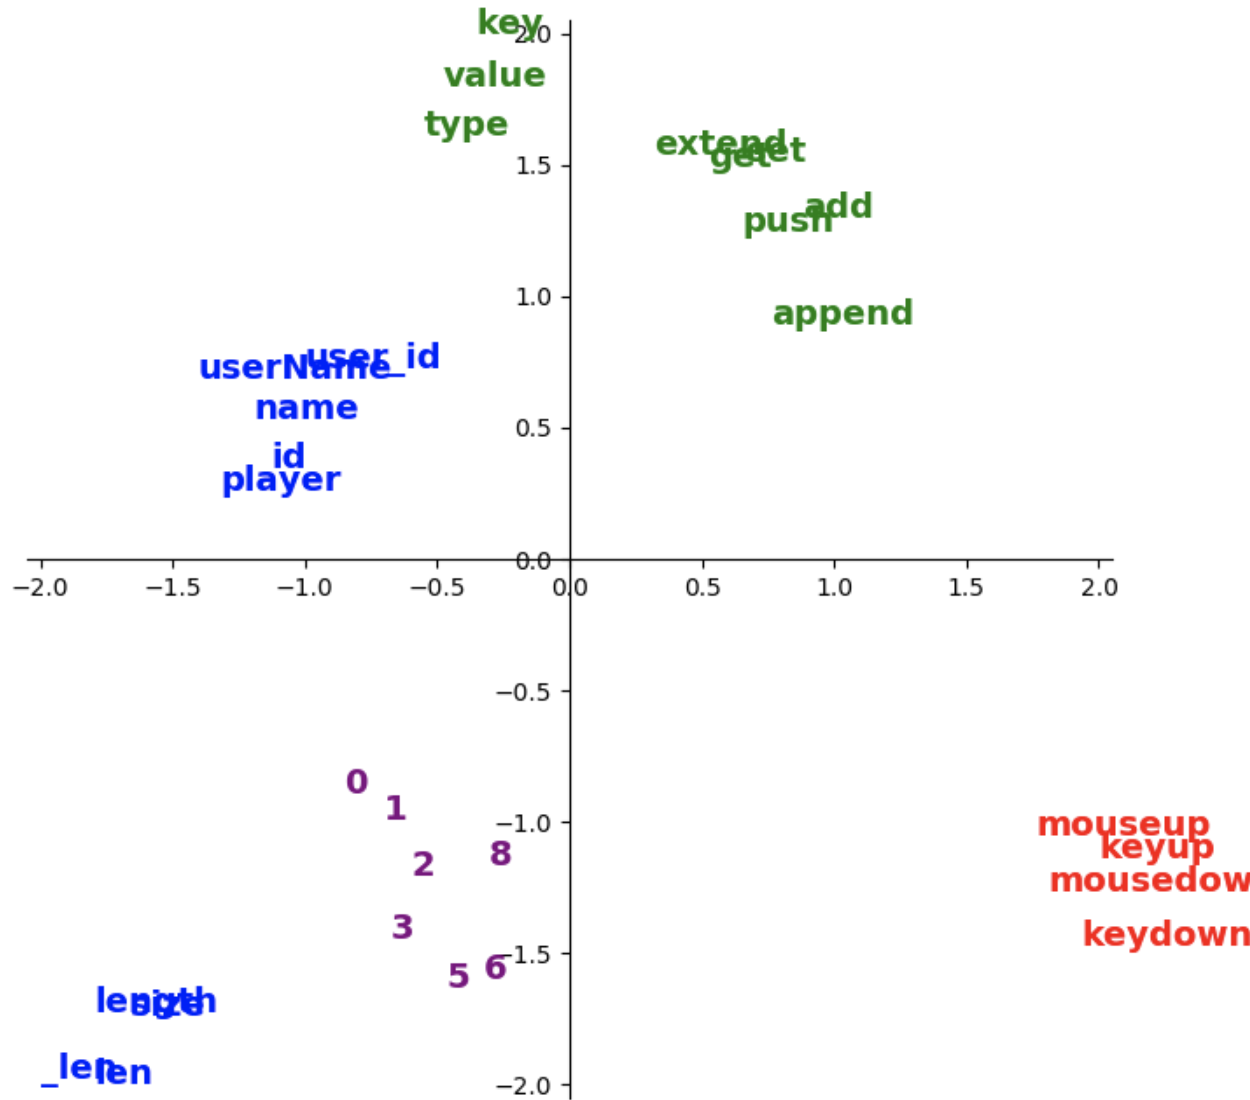
\includegraphics[scale=0.34]{pictures/node2vec_visualization.png}
\caption{The visualization of embedding vectors}
\label{fig:node2vec_visualization}
\end{figure}

In the figure, there are several clusters like: ``literal string cluster'', ``property cluster'' which represent different types of terminals. 
We also find that even tokens are the same type, if their meaning is different, they are still not in the same cluster. 
For example, even the type of ``append'' and ``value'' are \textit{Property}, they are still far from each other because ``append'' is a property which can add some elements to a container in the most cases.
However ``value'' usually is a member in a class without some operation functionality of a container. 
Another example is ``length'' and ``userName''.
Due to they have a different meaning, they are not in the same cluster even they are all \textit{Identifiers} 

% calculate similarity
We also calculate the cosine similarity between these embedding vectors and the result meets our conclusion of visualization. 
% The most similar token to ``identifier length'' is ``identifier size'' with the similarity 0.927 and the second similar token is ``identifier len'' with the similarity 0.883. 



\subsection{Experiment of AT2V-LSTM}
\subsubsection{Training details}
We implement two models for code completion: basic LSTM model and our AT2V-LSTM integration model to compare the predicting performance. 
We use Adam optimization algorithm to train our model with base learning rate 0.0025 and it multiplies 0.9 every epoch as learning rate decay. 
We clip the gradient which is more than 6 to 6 and less than -6 to -6 to avoid the gradient exploding problem.
We specify the time sequence $s=50$ and the batch size is $b=100$, therefore, there are $s \times b = 5000$ training instances for one training batch. 
We train two models $e=10$ epochs.

\subsubsection{Next Non-terminal Prediction} 
Valid accuracy curve of the next non-terminal token prediction during the training phase is illustrated in Figure \ref{fig:valid_accuracy_for_non_terminal}. 
The blue curve represents the validation accuracy of the basic LSTM model and the orange curve is our AT2V-LSTM integration model. 
%The x-axis is the validation checkpoint among training step, there are four checkpoints for each training epoch. Due to we train our models 10 epochs totally in the experiment, there are 40 checkpoints to record the validation accuracy. 

From the validation accuracy curves, we find the non-terminal prediction accuracy of AT2V-LSTM integration model is a little higher than the accuracy of the basic LSTM model. The evaluation result illustrated in the table\ref{table:non-terminal-evalution-accuracy} also shows that the accuracy of the integration model is 1.5\% higher than the basic baseline model. 

\begin{figure}[!ht]
\centering
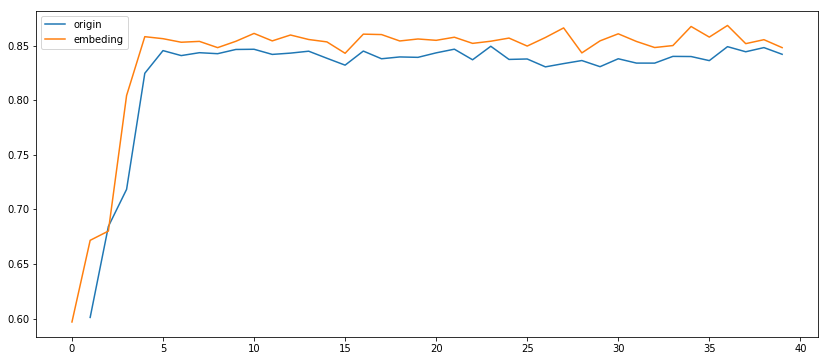
\includegraphics[scale=0.25]{pictures/nt_valid_accuracy.png}
\caption{Validation accuracy for non-terminal prediction during the training phase}
\label{fig:valid_accuracy_for_non_terminal}
\end{figure}



\begin{table}
\centering
\begin{tabular}{ccc}
\hline
Models& Top 1 accuracy& Top 3 accuracy\\
\hline
Basic LSTM& 83.5 $\pm$ 0.2\% & 92.6 $\pm$ 0.2\% \\
AT2V-LSTM& 85.2 $\pm$ 0.2\% & 94.4 $\pm$ 0.2\% \\
\hline
\end{tabular}
\caption{Non-terminal evaluation accuracy}
\label{table:non-terminal-evalution-accuracy}
\end{table}



\subsubsection{Next Terminal Prediction} 
Figure \ref{fig:valid_accuracy_for_terminal} illustrates the validation accuracy curve for next terminal token prediction during the training phase. 
Orange curve represents our AT2V-LSTM integration model and the blue curve is the accuracy of the basic LSTM model. 
The evaluation accuracy for the terminal in the test phase is shown in Tabel\ref{table:terminal-evalution-accuracy}. 
From both the evaluation result, we can find that the AT2V-LSTM integration model has a better performance with the predicting accuracy of 78.9\% than the basic baseline model 75.8\%. 


\begin{figure}[!ht]
\centering
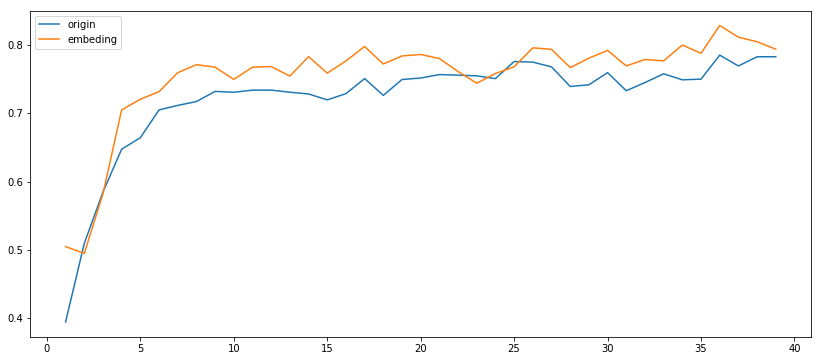
\includegraphics[scale=0.25]{pictures/tt_valid_accuracy.png}
\caption{Validation accuracy for terminal prediction during the training phase}
\label{fig:valid_accuracy_for_terminal}
\end{figure}


\begin{table}
\centering
\begin{tabular}{ccc}
\hline
Models& Top 1 accuracy& Top 3 accuracy\\
\hline
Basic LSTM& 75.8 $\pm$ 0.2\% & 87.7 $\pm$ 0.2\% \\
AT2V-LSTM& 78.9 $\pm$ 0.2\% & 89.2 $\pm$ 0.2\% \\
\hline
\end{tabular}
\caption{Terminal evaluation accuracy}
\label{table:terminal-evalution-accuracy}
\end{table}


\subsubsection{Next Token Information Prediction}
The evaluation result of the type (non-leaf or leaf) and the side (right-child or left-child) is shown in the Table\ref{table:node-information-evaluation-accuracy}.
We can find that both two models achieve a good performance that the accuracy of type information is near to 97\% and side information is near to 95\%. 


\begin{table}
\centering
\begin{tabular}{ccc}
\hline
Models& Type accuracy& Side accuracy\\
\hline
Basic LSTM& 97.6 $\pm$ 0.2\% & 94.8 $\pm$ 0.2\% \\
AT2V-LSTM& 97.8 $\pm$ 0.2\% & 95.1 $\pm$ 0.2\% \\
\hline
\end{tabular}
\caption{Type and side evaluation accuracy}
\label{table:node-information-evaluation-accuracy}
\end{table}

\subsubsection{Uncommon terminal repeation}
We analyze the possible reasons that may cause our integration model to work better for some evaluation cases. 

\begin{figure}[!ht]
\centering
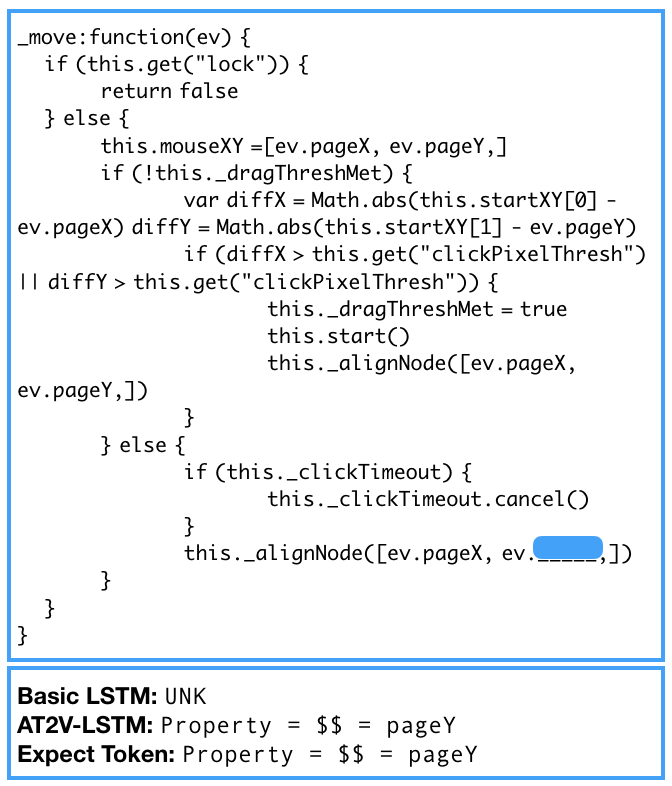
\includegraphics[height=8cm, width=7.4cm]{pictures/code_snippets_compare.png}
\caption{Code snippets for prediction result analysis}
\label{fig:code_snippets_compare}
\end{figure}


The code snippet in the figure\ref{fig:code_snippets_compare} is a test case and models predict what token should be filled in the hole.
The expecting token is ``Property pageY''.
The basic model predicts terminal ``UNK'' which means this model consider the token appearing in the hole is a quite uncommon terminal.
However, our AT2V-LSTM model gives a correct prediction.
From the programming habits and the statistic of the dataset, the ``property pageY'' is an uncommon terminal only appears in several files but repeats many times in one file. 
Due to it is uncommon, the basic LSTM model is hard o ltearn enough informatnio and give an incorrect prediction.
On the contrary, the AT2V-LSTM integration model can leverage the semantic information of ``pageY'' extracted by the ASTToken2Vec embedding and give a correct prediction.



\section{Conclusion}
In this paper, we propose an embedding method for AST nodes called ASTToken2Vec. 
We integrate it with a basic LSTM model to build an integration model called AT2V-LSTM.
From the results of our experiments, we conclude that the ASTToken2Vec model is able to generate the semantic-based embedding representation vectors for tokens.
These embedding vectors enable our AT2V-LSTM integration model to leverage more semantic knowledge hidden behind ASTs and to complete code with a higher possibility of predicting next tokens correctly. 
% We also extend the way to convert ASTs to sequences in the previous work with two more bits of information so that it is much easier to reconstruct a predicting AST from the sequence.



\bibliographystyle {jssst}
\bibliography {references}



\end{document}
